% empirical stats:  empirical_stats.tex
\begin{frame}
  \onslide<1->{
	\frametitle{Empirical Statistics} 
	\framesubtitle{Sample Means, Variances, etc.}
}
\begin{itemize}
  \onslide<2->{
\item Previously defined quantities $\mu_X,\sigma_X,\ldots$ were all theoretical properties, sometimes referred to 
as population statistics  
}
  \onslide<3->{
\item With real data we rarely know the true statistics;  we only have sampled data to go on  
}
  \onslide<4->{
\item But we can define quantities analogous to $\mu_X,\sigma_X,\ldots$ that we can actually compute 
using real data and that are generally in some sense approximations to the true values
}
\end{itemize}
\end{frame}
\begin{frame}
  \onslide<1->{
	\frametitle{Empirical Statistics} 
	\framesubtitle{Sample Means, Variances, etc.}
}
\begin{footnotesize}
\begin{itemize}
  \onslide<2->{
\item   With $N$ samples of random variable $X$, the \textbf{Sample Mean} is:  $$\samplemeandef{X}$$
}
  \onslide<3->{
\item The \textbf{Sample Variance} is: $$\samplevardef{X}$$  
}
  \onslide<4->{
\item  The \textbf{Sample Covariance} is: $$\samplecovdef{X}{Y}$$ 
}
  \onslide<5->{
\item   The \textbf{Sample Correlation} is: $$\samplecorrdef{X}{Y}$$
}
\end{itemize}
\end{footnotesize}
\end{frame}
\begin{frame}
  \onslide<1->{
	\frametitle{Empirical Statistics} 
	\framesubtitle{Sample Stats with MATLAB}
}
\begin{footnotesize}
True $\mu,\sigma$: mu=30;sigma=10;\\
1,000 samples:  X=mu+sigma*randn(1000,1);\\
$\samplemean{X}=29.6737$ and $\samplevar{X}=99.7932$ (sample standard deviation $s_X=9.9897$)\\
\begin{center}
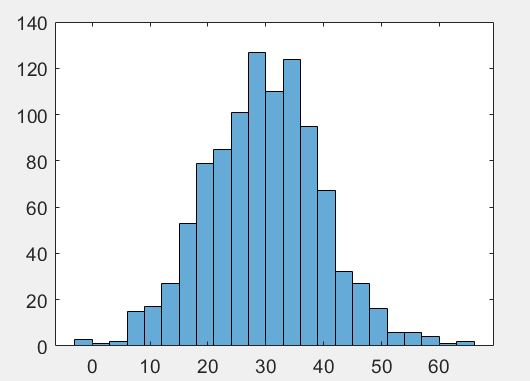
\includegraphics[scale=0.80]{day2_seg1_prob/histogram.jpg}
\end{center}
\end{footnotesize}
\end{frame}

\begin{frame}
  \onslide<1->{
	\frametitle{Empirical Statistics} 
	\framesubtitle{Sample Stats with MATLAB}
}
\begin{footnotesize}
True $\mu,\sigma$: mu=30;sigma=10;\\
10,000 samples: X=mu+sigma*\text{randn}(10000,1);\\
$\samplemean{X}=30.0563$ and $\samplevar{X}=97.3913$ (sample standard deviation $s_X=9.8687$)\\
\begin{center}
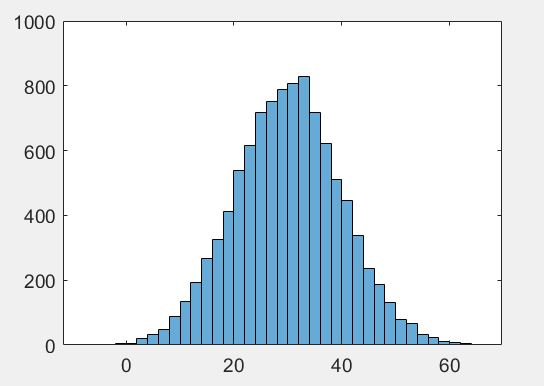
\includegraphics[scale=0.80]{day2_seg1_prob/histogram10000.jpg}
\end{center}
\end{footnotesize}
\end{frame}

\begin{frame}
  \onslide<1->{
	\frametitle{Empirical Statistics} 
	\framesubtitle{Sample Stats with MATLAB}
}
\begin{footnotesize}
True $\mu,\sigma$: mu=30;sigma=10;\\
10,000 samples: X=mu+sigma*\text{randn}(10000,1);\\
$\samplemean{X}=30.0563$ and $\samplevar{X}=97.3913$ (sample standard deviation $s_X=9.8687$)\\
\begin{center}
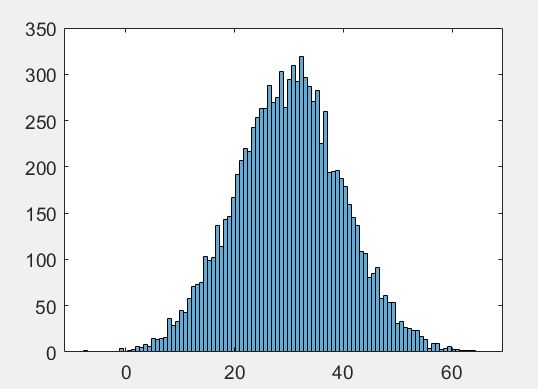
\includegraphics[scale=0.80]{day2_seg1_prob/histogram10000more_bins.jpg}
\end{center}
\end{footnotesize}
\end{frame}

\begin{frame}
  \onslide<1->{
	\frametitle{Empirical Statistics} 
	\framesubtitle{Sample Stats with MATLAB}
}
\begin{footnotesize}
True $\mu,\sigma$: mu=30;sigma=10;\\
10,000 samples: X=mu+sigma*randn(10000,1);\\
$\samplemean{X}=30.0563$ and $\samplevar{X}=97.3913$ (sample standard deviation $s_X=9.8687$)\\
$\;\;\;$\\
Define new random variable $Y$ to be linearly dependent on $X$ plus 
some random Gaussian noise:Y=3*X+2+randn(10000,1);\\
$\;\;\;$\\
MATLAB's corrcoef functions says (rightly) that $X$ and $Y$ are highly correlated: $r_{XY}=0.9994$
\end{footnotesize}
\end{frame}
